\documentclass[tikz,border=8pt]{standalone}
% Shared look for every TikZ diagram. Load with \input{../../tools/tikz-style.tex}
\usepackage[T1]{fontenc}
\usepackage{lmodern}
\renewcommand{\sfdefault}{lmr}  % diagrams use the same serif as the text
\usetikzlibrary{arrows.meta, positioning, shapes.geometric, calc, fit, backgrounds}
\definecolor{cblue}{HTML}{4C78A8}
\definecolor{corange}{HTML}{F58518}
\definecolor{cgreen}{HTML}{54A24B}
\definecolor{cred}{HTML}{E45756}
\definecolor{cpurple}{HTML}{B279A2}
\definecolor{cgrey}{HTML}{6B6B6B}
\tikzset{
  every picture/.style={font=\sffamily, line width=1.2pt},
  box/.style={draw=#1, fill=#1!12, rounded corners=4pt, align=center, inner sep=7pt, minimum height=1.1cm},
  box/.default=cgrey,
  arrow/.style={-{Stealth[length=3mm]}, draw=cgrey, line width=1.4pt},
  title/.style={font=\sffamily\bfseries\Large},
  note/.style={font=\sffamily\small, text=cgrey, align=center},
}
\AtBeginDocument{\hyphenpenalty=10000 \exhyphenpenalty=10000}

% One robot, two frames: measured from the room corner A it is at (2, 1); from the corner of a rug B at (1, 0.5)
% it is at (1, 0.5). Same robot, different numbers: a position needs its frame.
\begin{document}
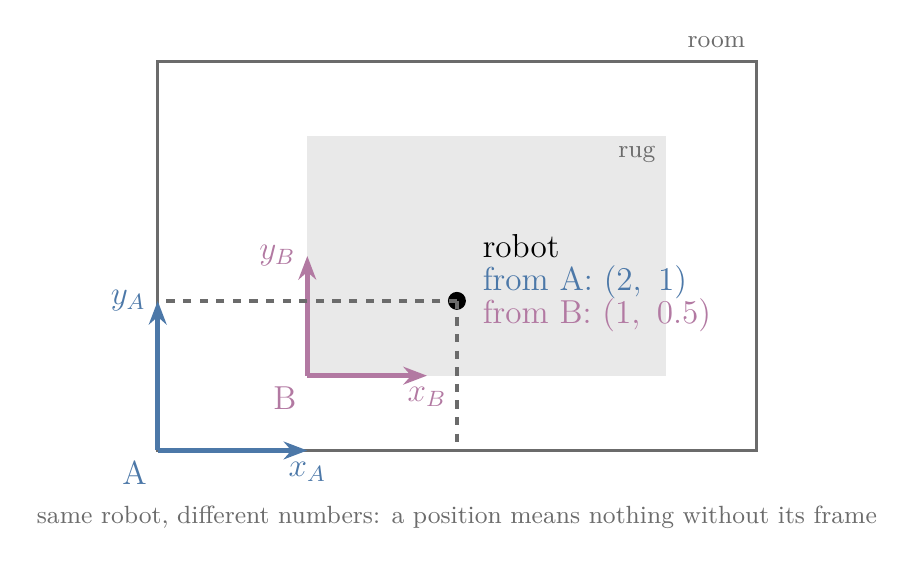
\begin{tikzpicture}[scale=1.9, every node/.append style={font=\large}]
  \draw[cgrey, line width=1pt] (0,0) rectangle (4,2.6);
  \node[note, anchor=south east] at (4,2.62) {room};
  \fill[cgrey!15] (1,0.5) rectangle (3.4,2.1);
  \node[note, anchor=north east] at (3.4,2.1) {rug};
  % frame A
  \draw[-{Stealth[length=3mm]}, cblue, line width=2pt] (0,0) -- (1.0,0) node[below] {$x_A$};
  \draw[-{Stealth[length=3mm]}, cblue, line width=2pt] (0,0) -- (0,1.0) node[left] {$y_A$};
  \node[cblue, below left] at (0,0) {A};
  % frame B
  \draw[-{Stealth[length=3mm]}, cpurple, line width=2pt] (1,0.5) -- (1.8,0.5) node[below] {$x_B$};
  \draw[-{Stealth[length=3mm]}, cpurple, line width=2pt] (1,0.5) -- (1,1.3) node[left] {$y_B$};
  \node[cpurple, below left] at (1,0.5) {B};
  % robot
  \fill[black] (2,1) circle (0.06);
  \draw[cgrey, dashed] (2,1) -- (2,0); \draw[cgrey, dashed] (2,1) -- (0,1);
  \node[right, align=left] at (2.1,1.12) {robot\\[-2pt]{\color{cblue}from A: $(2,\ 1)$}\\[-2pt]{\color{cpurple}from B: $(1,\ 0.5)$}};
  \node[note, anchor=north] at (2,-0.3) {same robot, different numbers: a position means nothing without its frame};
\end{tikzpicture}
\end{document}
